%
% kamera.tex
%
% (c) 2018 Prof Dr Andreas Müller, Hochschule Rapperswil
%
\section{Anwendung: Kamera-Geometrie\label{section:kamera}}
\index{Kamera}%
\index{Brennweite}%
Die rasante Entwicklung der Mikroelektronik und vor allem der
allgegenwärtigen Kameras in Mobiltelefonen hat dazu geführt, dass 
Bildsensoren heute klein, billig und mit wenig Software-Aufwand
einsetzbar sind.
Zwar muss für die Verarbeitung der ein etwas höherer Aufwand geleistet
werden, doch die ebenfalls gestiegene Prozessorleistung ermöglicht
Bildanalysen, die vor wenigen Jahren noch undenkbar waren.
Standard-Schnittstellen und Bibliotheken für die Bildverarbeitung
haben Kameras sind zu Allzweck-Sensoren geworden.
Mit der gleichen, massenproduzierbaren Hardware können mit
verschiedener Software die unterschiedlichsten Anwendungsprobleme
gelöst werden.

Kameras können zum Beispiel verwendet werden, um Objekte im Raum
zu lokalisieren.
Dazu muss die Software die Objekte im Bild erst finden.
Die klassische Bildverarbeitung hat auf diese Aufgabe spezialisierte
Methoden entwickelt.
Wir können also davon ausgehen, dass wir die Pixel-Koordinaten eines
Objektes aus einem Bild herauslesen können.
Die geometrische Aufgabe, die jetzt gelöst werden muss, ist, die
Raumkoordinaten des Objektes zu bestimmen.
Mit nur einer Kamera ist das natürlich nicht möglich, im besten Fall kann
eine Gerade bestimmt werden, auf der das Objekt zu finden ist.
Mit zusätzlichen Kameras kann dann mittels Triangulation eine mehr
oder weniger genaue Position bestimmt werden.

Das umgekehrte Problem ist etwas einfacher: Gegeben ein Punkt im Raum,
finde die Pixelkoordinaten, auf die der Punkt durch die Kamera
abgebildet wird.
Um diese Aufgabe zu lösen, muss man natürlich einiges über die Kamera
wissen.
Zum Beispiel sollte die Kamera ungefähr auf das Objekt ausgerichtet sein,
wir brauchen also Position und Orientierung der Kamera.
Die Brennweite hat einen Einfluss auf des Gesichtsfeld der Kamera.

In den folgenden Abschnitten wird schrittweise ein Formalismus
aufgebaut, mit dem sich alle diese Probleme mit den Werkzeugen der
linearen Algebra behandeln lassen.

%
% funktion.tex
%
% (c) 2018 Prof Dr Andreas Müller, Hochschule Rapperswil
%
\subsection{Funktion einer Kamera\label{subsection:kamerafunktion}}
Ziel dieses Abschnitts ist, eine Abstraktion einer Kamera zu finden,
welche sich einerseits geometrische einfach analysieren lässt aber
andererseits ein gutes Modell für eine genügend grosse Klasse von
real existierenden Kameras ist.
Komplizierter gebaute Kameras können dann wenn nötig durch Erweiterung dieses
Grundmodells beschrieben werden.
\subsubsection{Aufbau einer Kamera}
\begin{figure}
\centering
\includegraphics{applications/kamera/kamera.pdf}
\caption{Wichtigste Komponenten einer Kamera. Im roten Kameragehäuse befindet
sich der Bildsensor-Chip mit seiner Steuer- und Interface-Elektronik.
Das Bild wird vom Objektiv auf dem Chip erzeugt.
\label{applications:kamera:kamera-bild}}
\end{figure}
\begin{figure}
\centering
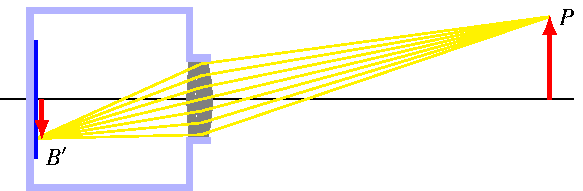
\includegraphics{applications/kamera/kameraprinzip.pdf}
\caption{Funktionsweise einer Kamera. Das Objektiv fokusiert den
Weltpunkt $P$ in den Bildpunkt $B$ auf dem Bildsensor ({\color{blue}blau}).
\label{applications:kamera:kameraprinzip}}
\end{figure}
Abbildung~\ref{applications:kamera:kamera-bild} zeigt die beiden in unserem
Zusammenhang wesentlichen Komponenten einer Kamera.
Das Objektiv fokusiert das von den abzubildenden Objekten ausgestrahlte
Licht und formt so ein Bild auf der Ebene des Bildsensors.
Eine Steuer- und Interface-Elektronik liest die Bilddaten aus dem Chip
aus, digitalisiert sie und macht sie zum Beispiel über ein USB-Interface
für einen Computer zugreifbar.
Einem Weltpunkt $P$ im dreidimensionalen Raum wird auf diese Weise ein
Bildpunkt $B$ auf der Chip-Ebene zugeordnet.

Die Qualität des erzeugten Bildes wird wesentlich bestimmt durch das
Objektiv.
Je grösser seine Öffnung ist, desto mehr Licht steht auf dem Chip zur
Verfügung.
Eine grosse Öffnung macht es aber auch schwierig, eine scharfe Abbildung
zu erreichen.
Die Lichtstrahlen am Rand einer grossen Linse werden nicht in den gleichen
Brennpunkt fokusiert wie die Strahlen, die die Linse Nahe dem Zentrum
passieren.
Mit einem einfachen zweilinsigen Objektiv wie in
Abbildung~\ref{applications:kamera:kamera-bild} ist das Bild nur nahe
der optischen Achse wirklich scharf.
Moderne Objekte verwenden daher mindestens vier oder noch mehr Linsen,
oder sogar Linsen, deren Oberfläche nicht sphärisch geschliffen ist.

\begin{figure}
\centering
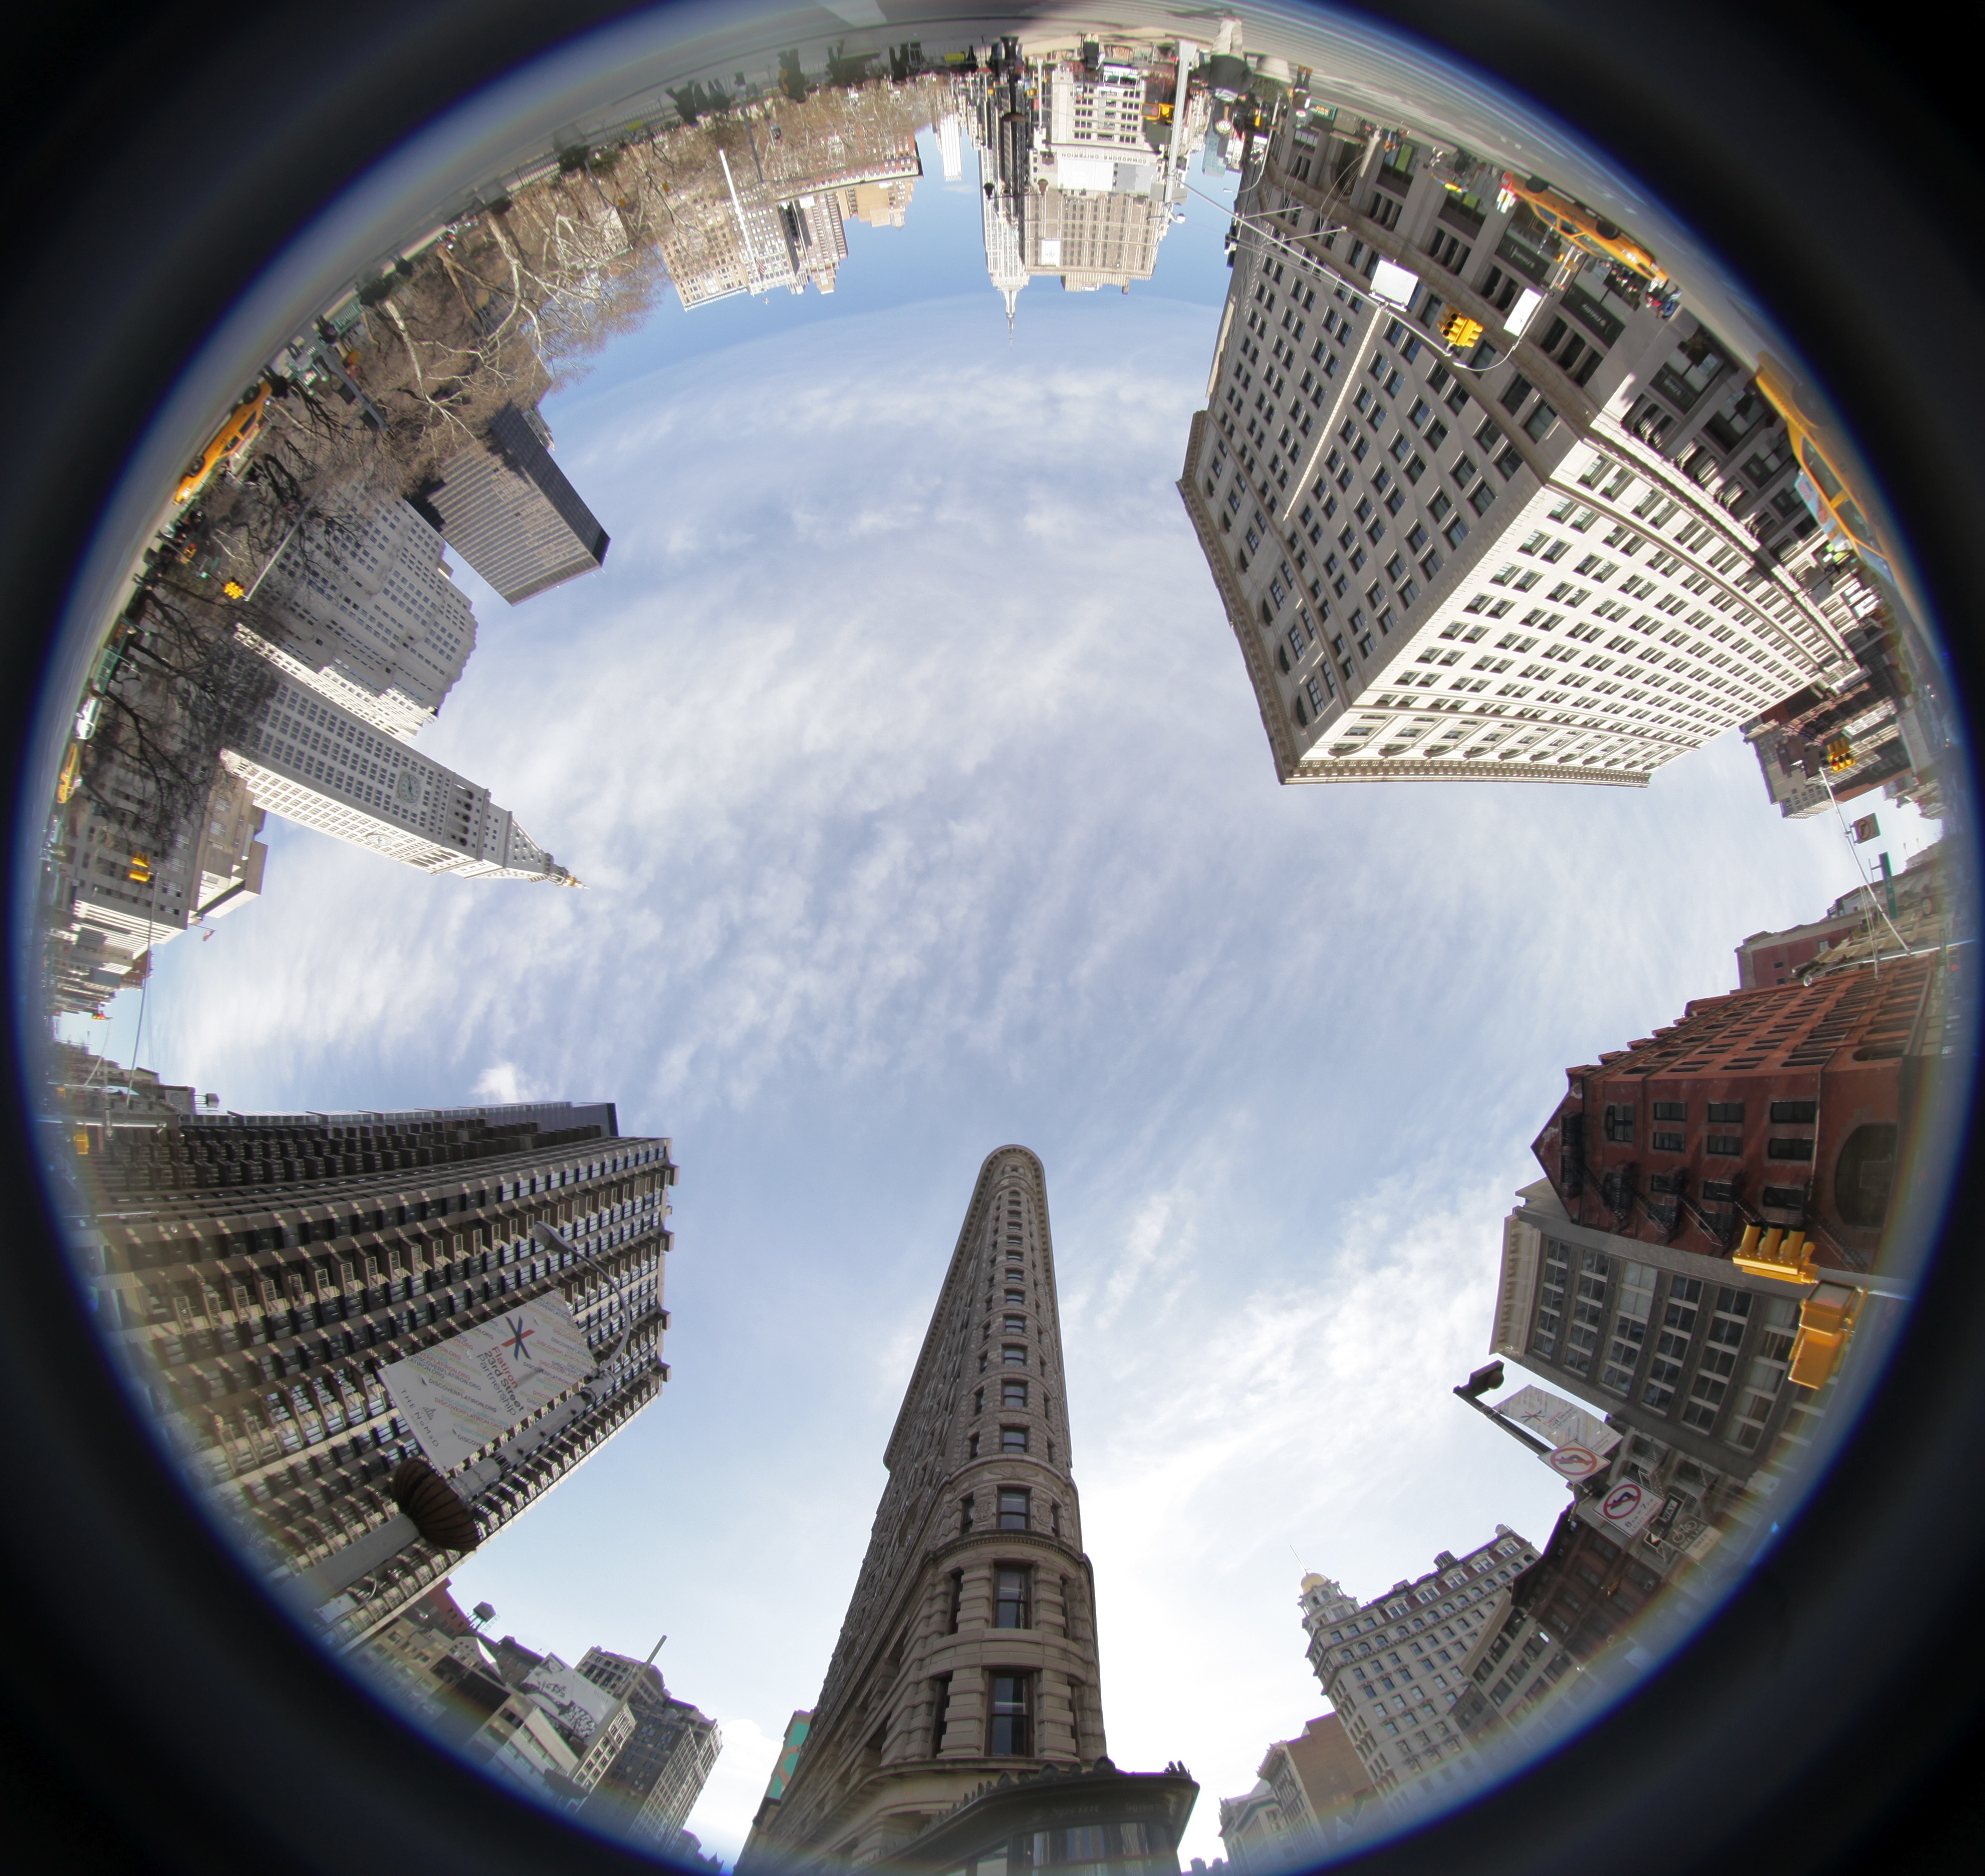
\includegraphics[width=8cm]{applications/kamera/fisheye.jpg}
\caption{Ein Fischauge-Objektiv bildet eine $180^\circ$-Gesichtsfeld in
einen Kreis ab.
Dabei werden Geraden in gekrümmte Linien abgebildet.
\label{applications:kamera:fisheye}}
\end{figure}%
Objektive sehr kurzer Brennweite können oft nicht ohne radiale Verzerrungen
gebaut werden.
Besonders ausgeprägt ist dies bei den Fischauge-Objektiven
(Abbildung~\ref{applications:kamera:fisheye}), die
ein Gesichtsfeld von $180^\circ$ in einen Kreis abbilden können.
Sie zeichnen sich dadurch aus, dass Geraden im Raum auf gekrümmte
Linien auf dem Bild abgebildet werden, solche Objektive lassen sich
also nicht mit einer linearen Abbildung beschreiben.

\subsubsection{Lochkamera}
Um die Analyse der Kameraabbildung zu vereinfachen stellen wir uns vor,
dass der Durchmesser des Objektivs immer kleiner gemaht wird.
Die Abbildungsfehler, die durch die Krümmung der Linse in den Randzonen
hervorgerufen wird, fallen dann weg.
Die Linse wirkt dann nur noch wie ein winzig kleines Loch, die Krümmung
der Linse ist nicht mehr von Bedeutung.
\begin{figure}
\centering
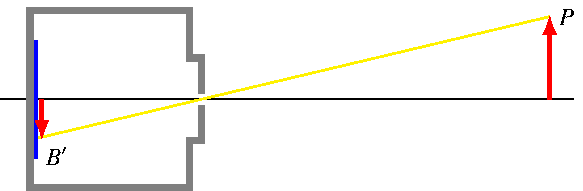
\includegraphics{applications/kamera/lochkamera.pdf}
\caption{Vereinfachung der Kamera von
Abbildung~\ref{applications:kamera:kameraprinzip} zu einer Lochkamera
\label{applications:kamera:lochkamera}}
\end{figure}
Eine solche Lochkamera ist ein vereinfachtes Modell für Kameras mit
nicht zu kurzer Brennweite.

Die Abbildung einer Lochkamera ist geometrisch sehr einfach.
Ein vom Weltpunkt $P$ ausgehender Lichtstrahl verläuft in gerader
Linie durch das Loch und schneidet die Chip-Ebene im Bildpunkt $B$.
Eine Gerade $g$ im Raum wird von einer Schar von Geraden durch das Loch und
die Geraden $g$ abgebildet.
Diese Geraden liegen alle in einer Ebene $\sigma$.
Die zugehörigen Bildpunkt liegen daher auf der Schnittgeraden der
Chip-Ebene mit der Ebene $\sigma$ der Abbildungsstrahlen.
Insbesondere bildet die Lochkamera Geraden immer wieder in Geraden ab.
Wir erwarten daher, dass diese Abbildung mit Hilfe von Matrizen
beschrieben werden kann.

%
% homogen.tex -- homogene Koordinaten
%
% (c) 2018 Prof Dr Andreas Müller, Hochschule Rapperswil
%
\subsection{Homogene Koordinaten\label{section:homogene koordinaten}}
Wir wollen das Abbildungs-Problem für eine einzelne Kamera lösen.
Ein Punkt im dreidimensionalen Raum wird durch seine drei Koordinaten
$(x,y,z)$ beschrieben.
Wir nennen einen solchen Punkt auch {\em Weltpunkt} und seine Koordinaten
die {\em Weltkoordinaten}.
\index{Weltpunkt}%
\index{Weltkoordinaten}%
Er wird abgebildet auf einen {\em Bildpunkt} auf dem Kamera-Chip mit
Pixel-Koordinaten, auch {\em Bildkoordinaten}.
\index{Bildpunkt}%
\index{Bildkoordinaten}%
\begin{aufgabe}[Abbildungsproblem für Kameras]
Gegeben die Koordinaten eines Weltpunktes, berechne die Bildkoordinaten
für eine beliebige Kamera.
\end{aufgabe}
Es ist klar, dass alle Punkte auf einem Strahl durch die Kamera auf den
gleichen Bildpunkt abgebildet werden.
Gesucht ist also eine mathematische Beschreibung, die solche Strahlung
zu beschreiben gestattet.
Dies sind die {\em homogenen Koordinaten}.

\subsubsection{Strahlensatz}
\begin{figure}
\centering
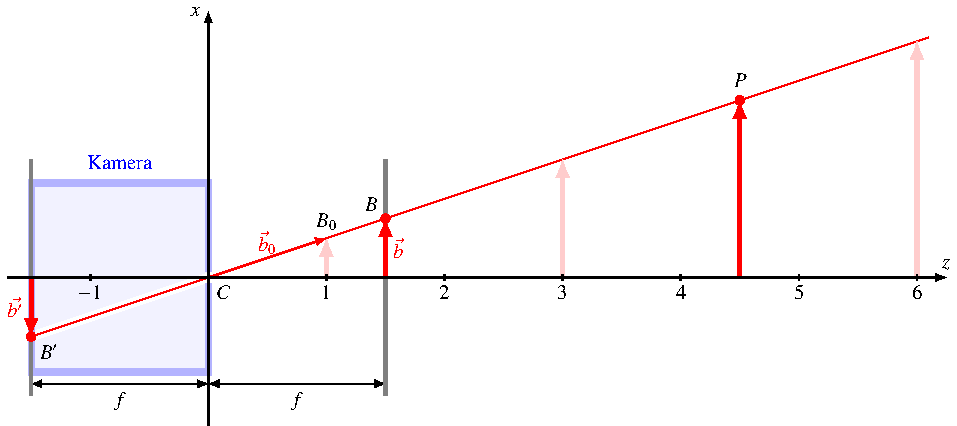
\includegraphics{applications/kamera/strahlensatz.pdf}
\caption{Strahlensatz und Abbildung eines Punktes $P$ durch eine Lochkamera
mit Brennweite $f$.
\label{skript:kamera:strahlensatz}}
\end{figure}
In Abbildung~\ref{skript:kamera:strahlensatz} ist illustriert, wie
der Punkt $P$ durch die blau angedeutete Lochkamera auf den Punkt $B'$
abgebildet wird.
Das Loch befindet sich im Punkt $C$ und die Kamera hat die Brennweite $f$.
Der Pfeil von der $z$-Achse zum Punkt $P$ der Länge $x(z)$ wird
auf den kopfstehenden Pfeil von der $z$-Achse zum Punkt $B'$ abgebildet.
Das Abbildungsproblem ist gelöst, wenn wir die Länge des Vektors $\vec{b'}$
bestimmen können.
Da $\vec{b}'=-\vec{b}$ ist, ist das gleichbedeutend damit, den Vektor $\vec{b}$
zu bestimmen.

Alle Punkte auf der roten Geraden durch $C$ und $P$ werden von der Kamera
auf den gleichen Punkt $B'$ abgebildet.
Die Gerade besteht aus den Punkte mit Ortsvektoren, die Vielfache des
Vektors $\vec{b}_0=\overrightarrow{CB_0}$ sind.
Alle Punkte sind also Vielfache des Vektors 
\[
\vec{b}_0
=
\overrightarrow{CB_0}
=
\begin{pmatrix}x(B_0)\\1\end{pmatrix}.
\]
Auch der Ortsvektor des Bildpunktes $B$ in der Fokusebene ist ein Vielfaches 
von $\vec{b}_0$, nämlich
\[
\overrightarrow{CB}
=
\begin{pmatrix}x(B)\\f\end{pmatrix}
=
f \cdot
\begin{pmatrix}x(B_0)\\1\end{pmatrix}.
\]
Unabhängig von der Brennweite können also alle Bildpunkte durch 
den Vektor $\vec{b}_0$ dargestellt werden.
Dies suggeriert, dass wir als Koordinatensystem für die Punkte in der
Brennebene nicht einfach nur die Länge der Strecke von der $z$-Achse 
zum Punkt $B$ verwenden sollen, sondern zweidimensionale Vektoren.
Die Länge der genannten Strecke finden wird dann, indem wir den Vektor
so skalieren, dass die zweite Komponente $f$ wird.

Die Idee, dass skalierte Vektoren das gleiche geometrische Objekt
beschreiben, führt uns auf den Begriff der {\em homogenen Koordinaten}%
\index{homogene Koordinaten}%
.
Wir beginnen damit zu zeigen, wie homogene Koordinaten die Punkte
einer Geraden beschreiben können.
Anschliessend verwallgemeinern wir die Idee darauf, Punkte der Bildebene
und des dreidimensionalen Raumes mit homogenen Koordinaten zu beschreiben.

\begin{definition}
Wir nennen Zahlenpaare $(x_1,x_2)$ {\em homogene Koordinaten} für die
Punkte einer Geraden, wenn mindestens eine der Komponenten von $0$
verschieden ist (Abbildung~\ref{applications:kamera:homogenekoordinaten}).
Die inhomogene (gewöhnlichen) Koordinate eines Punktes mit
homogenen Koordinaten $(x_1,x_2)$ mit $x_2\ne 0$ ist $x_1/x_2$.
\end{definition}
\index{homogene Koordinaten}%
\begin{figure}
\centering
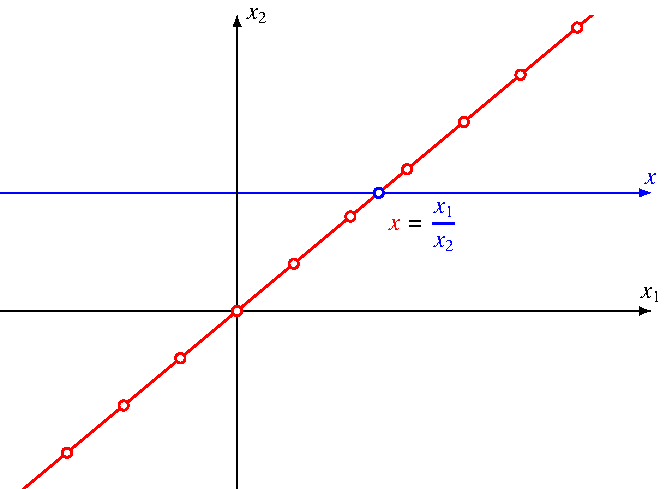
\includegraphics{applications/kamera/homogenekoordinaten.pdf}
\caption{Homogene Koordinaten für die Punkte auf der $x$-Achse
({\color{blue}blau}) sind Paare $(x_1,x_2)$.
Die Punkte {\color{red}$(x_1,x_2)$} mit gleichem Verhältnis $x_1/x_2$
liegen auf einer
Geraden in der $x_1$-$x_2$-Ebene und beschreiben den gleichen Punkt
$\color{blue}x$.
\label{applications:kamera:homogenekoordinaten}}
\end{figure}
Man beachte, dass den homogenen Koordinaten $(1,0)$ keine gewöhnliche
Koordinate zugeordnet ist.
Sie beschreiben einen Punkte auf der $x$-Achse von
Abbildung~\ref{skript:kamera:strahlensatz}.
Doch dieser Punkt kann von der Kamera gar nicht abgebildet werden.
Man nennt diesen Punkt manchmal auch den {\em unendlich fernen Punkt} der
Geraden.
\index{unendlich ferner Punkt}%

In homogenen Koordinaten lässt sich das Abbildungsproblem also ganz
einfach lösen. 
Der Punkt $P$ mit Koordinaten $(x,z)$ wird abgebildet auf den Punkt
mit homogenen Koordinaten $(x,z)$.
Um die inhomogene Koordinate mit in einer Kamera mit Brennweite $f$ zu
berechnen, setzen wir einfach $f\cdot x/z$ ein.

Auf den Mittelpunkt des Bildes werden alle Punkte der $z$-Achse
in Abbildung~\ref{skript:kamera:strahlensatz} abgebildet.
Die homogenen Koordinaten dieses Punktes sind $(0,1)$, dies ist
auch der Richtungsvektor der Blickrichtung der Kamera.

\subsubsection{Zentralprojektion auf eine Ebene}
Bisher haben wir eine eindimensionale Kamera studiert.
Dafür gibt es durchaus bereits Anwendungen, zum Beispiel Scanner
mit linearem Bildsensor.
Aber natürlich interessieren uns vor allem realistischere Kameras
mit zweidimensionalem Sensor.
Dazu müssen wir das Konzept der homogenen Koordinaten auf einen
dreidimensionalen Raum ausdehen.

\begin{definition}
Wir nennen Zahlentripel $(x_1,x_2,x_3)$ {\em homogene Koordinaten}
für die Punkte einer Ebene, wenn mindestens eine der Komponenten von $0$
verschieden sind.
Die inhomogenen Koordinaten eines Punktes mit homogenenen Koordinaten
$(x_1,x_2,x_3)$ mit $x_3\ne 0$ sind $(x_1/x_3,x_2/x_3)$.
\end{definition}

Wir stellen uns also wieder vor, eine Lochkamera im Ursprung des
Koordinatensystems platziert zu haben mit Blickrichtung entlang der
$z$-Achse.
Die inhomogenen Koordinaten des Punktes $P=(x,y,z)$ können wir dann
wieder als homogene Koordinaten einer Ebene betrachten.
Die Abbildung durch die Lochkamera mit Brennweite ist dann wieder sehr
einfach zu lösen: der Punkt $P$ wird auf den Punkt mit homogenen Koordinaten
$(x,y,z)$ abgebildet.
Die Koordinaten in der Brennebene einer Kamera mit Brennweite $f$ sind dann
$f\cdot (x/z, y/z)$.

Die Punkte mit $z=0$ können nicht abgebildet werden.
Wenn die $z$-Koordinaten eines Punktes gegen $0$ geht, bewegt sich sein
Bild in der Brennebene der Lochkamera nach aussen gegen unendlich.
Man nennt diese Punkte daher manchmal auch unendlich ferne Punkte.
Da sie ausserdem eine lineare Gleichung erfüllen, kann man die Menge dieser
Punkte auch die {\em unendlich ferne Gerade} nennen.
\index{unendlich ferne Gerade}%

\subsubsection{Umrechnung in homogene Koordinaten}
Nach dem gleichen Muster wie in einer und zwei Dimensionen
können wir von jedem $n$-dimensionalen Raum homogenen Koordinaten einführen.
Der Übergang von homogenen Koordinaten geschieht dabei durch Division
durch die letzte Koordinate.
Der Übergang in der umgekehrten Richtung werden wir später wiederholt
brauchen und führen daher folgende Notation ein.

\begin{definition}
Einem Punkt mit inhomogenen Koordinaten $x=(x_1,x_2,\dots,x_{n})\in\mathbb R^n$
entspricht ein Punkt mit inhomogenen Koordinaten
\[
\tilde x = (x_1,x_2,\dots,x_{n},1) \in \mathbb R^{n+1}.
\]
\end{definition}


%%
% kmatrix.tex
%
% (c) 2018 Prof Dr Andreas Müller, Hochschule Rapperswil
%
\subsection{Kamera-Spezifikation\label{section:kameraspez}}
Die im Abschnitt~\ref{section:homogene koordinaten} beschriebene
Lösung des Abbildungsproblems bildet die Punkte auf der Kameraachse
auf den Nullpunkt der Brennebene ab.
Der Chip einer realen Kamera ist dagegen nur ein Rechteck, 
welches üblicherweise mit einem Koordinatensystem ausgestattet wird,
welches den Nullpunkt in einer Ecke hat.
Als Masseinheit werden ausserdem meistens Pixel verwendet, nicht die
Masseinheiten, die für Weltpunkte verwendet werden.
Dieser Chip wird meistens so montiert, dass die Achse der Kamera
durch den Mittelpunkt des Chips geht.
Wir brauchen daher eine Umrechnungsformel, welche die homogenen
Koordinaten des Bildpunktes in die Chip-Koordinaten umrechnet.

\subsubsection{Brennweite und Pixelkoordinaten}
\begin{figure}
\centering
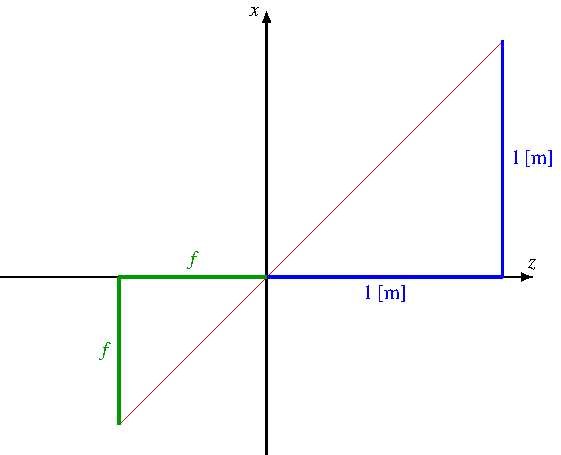
\includegraphics{applications/kamera/brennweite.pdf}
\caption{Brennweite und Umrechnung in Pixelkoordinaten (siehe Text)
\label{skript:kamera:brennweite}}
\end{figure}
Zunächst untersuchen wir nochmals die Bedeutung der Brennweite $f$.
Die Kamera bildet den Punkt $(x,y,z)$ zunächst auf die homogenen
Koordinaten $(x,y,z)$ ab.
Zur Bestimmung der inhomogenen Koordinaten in der Brennebene 
berechnen wir zunächst $(x/z, y/z)$.
Dies entspricht der Projektion in die Brennebene mit $z=1$,
dies gilt aber für $z$ gemessen in den Masseinheiten des
Weltkoordinatensystems.
Wir brauchen nun aber die Umrechnung in Pixel-Koordinaten im Bild,
und verwenden dazu die Abbildung~\ref{skript:kamera:brennweite}.
Wir lesen daraus ab, dass ein Punkt mit homogener Koordinate $(1,1)$
abgebildet wird auf einen Punkt mit inhomgenen Pixelkoordinaten $f$
abgebildet.

In drei Dimensionen bedeutet das, dass der Punkt mit Koordinaten
$(x,y,z)$ abgebildet wird auf den Punkt
\[
(x,y,z) \mapsto (f\cdot x/z, f\cdot y/z).
\]
In Matrixschreibweise ist dies die Folge von Abbildungen
\[
\begin{pmatrix}
x\\y\\z
\end{pmatrix}
\mapsto
\begin{pmatrix}
x/z\\y/z
\end{pmatrix}
\mapsto
\begin{pmatrix}
f\cdot x/z\\f\cdot y/z
\end{pmatrix}.
\]
Die erste Abbildung lässt sich nicht als Matrix schreiben.
Wir könnten aber auf die Divison verzichten und stattdessen
die dritte Komponente $z$ behalten und erst am Schluss durch $z$
dividieren:
\[
\begin{pmatrix}
x\\y\\z
\end{pmatrix}
\mapsto
\begin{pmatrix}
f\cdot x\\f\cdot y\\z
\end{pmatrix}
=
\begin{pmatrix}
f&0&0\\
0&f&0\\
0&0&1
\end{pmatrix}
\begin{pmatrix}
x\\y\\z
\end{pmatrix}
\mapsto
\begin{pmatrix}
f\cdot x/z\\f\cdot y/z
\end{pmatrix}.
\]
Die Skalierung mit der Brennweite wird also am besten mit Hilfe der
Matrix
\[
K_f
=
\begin{pmatrix}f&0&0\\0&f&0\\0&0&1\end{pmatrix}
\]
in homogenen Koordinaten beschrieben.

\subsubsection{Kameraachse und Verschiebung}
Die Achse der Kamera geht durch den Mittelpunkt $(m_x,m_y)$ des Chips.
Punkte der Achse haben homogenen Koordinaten $(0,0,z)$, sollten aber
auf $(m_x,m_y)$ abgebildet werden.
Wir müssen also den inhomogenen Koordinaten noch die Komponenten
$m_x$ und $m_y$ hinzufügen, nämlich
\[
\begin{pmatrix} x/z \\ y/z \\ 1 \end{pmatrix}
\mapsto
\begin{pmatrix} x/z +m_x\\ y/z +m_y\\ 1 \end{pmatrix}.
\]
Dies können wir ebenfalls als Matrix beschreiben:
\[
\begin{pmatrix} x/z +m_x\\ y/z +m_y\\ 1 \end{pmatrix}.
=
\underbrace{
\begin{pmatrix}
1&0&m_x\\
0&1&m_y\\
0&0&1
\end{pmatrix}
}_{\displaystyle K_m}
=
\begin{pmatrix} x/z \\ y/z \\ 1 \end{pmatrix}.
\]
Natürlich können wir auch wieder mit $z$ multiplizieren, die Matrix
$K_m$ beschreibt die Translation um $(m_x,m_y)$ auch in homogenen
Koordinaten.

\subsubsection{Die Kameramatrix $K$}
Die Matrix $K_f$ beschreibt die Wirkung der Brennweite in homogenen
Koordinaten, während die Matrix $K_m$ die Wirkung der Translation um
$(m_x,m_y)$ in homogenen Koordinaten beschreibt.
Die Wirkung der Kamera kann daher zusammengefasst werden in eine einzige
Matrix
\[
K
=
K_m\cdot K_f
=
\begin{pmatrix}
1&0&m_x\\
0&1&m_y\\
0&0&1
\end{pmatrix}
\begin{pmatrix}
f&0&0\\
0&f&0\\
0&0&1
\end{pmatrix}
=
\begin{pmatrix}
f&0&m_x\\
0&f&m_y\\
0&0&1
\end{pmatrix},
\]
die {\em Kameramatrix}.
\index{Kameramatrix}%

\subsubsection{Weitere kamerainterne Einflüsse}
TODO: Chipneigung, nicht quadratische Pixel, Kalibrierung




%%
% drehung.tex
%
% (c) 2018 Prof Dr Andreas Müller, Hochschule Rapperswil
%
\subsection{Kameraorientierung und Kamerazentrum\label{section:kameraorientierung}}
Bis jetzt war die Kamera im Nullpunkt des Koordinatensystems platziert
und die Achse der Kamera war parallel zur $z$-Achse, die $x$-Achse des Chips
horizontal.
Eine Kamera kann aber in jedem beliebigen Punkt $c$, dem Kamerazentrum,
des Raumes platziert sein und die Achsen der Kamera können beliebig gegenüber
dem Standard-Koordinatensystem verdreht sein.
Um das Abbildungsproblem zu lösen, müssen wir also die Weltpunkte erst
umrechnen in das Koordinatensystem der Kamera, bevor wir die Kameramatrix
darauf anwenden können.

\subsubsection{Kamerazentrum}
Die Kamera befindet sich im Punkt mit dem Ortsvektor $c$ statt dem
Nullpunkt.
Statt die Kamera in den Nullpunkt zu verschieben, können wir auch die
Position des abzubildenden Weltpunktes $P$ um $c$ korrigieren.
Für eine Kamera im Punkt $c$ sieht der Nullpunkt genau so aus wie
der Punkt $-c$ für eine Kamera im Nullpunkt.
Wir müssen also die Translation $p\mapsto p-c$ durchführen.
Leider ist dies keine lineare Abbildung.
Wir können aber wie bereits bei der Diskussion der Kameramatrix $K_m$
gesehen, dass dies in homogenen Koordinaten ganz einfach geht.
Wir schreiben daher Weltpunkte mit inhomogenen Koordinaten
$(x,y,z)$ als als Quadrupel von homogenen Koordinaten $(x,y,z,1)$.
Damit können wir die Translation schreiben als
\[
p \mapsto p-c =
\begin{pmatrix}
1&0&0&-c_x\\
0&1&0&-c_y\\
0&0&1&-c_z
\end{pmatrix}
\begin{pmatrix}
x\\y\\z\\1
\end{pmatrix}
=
\begin{pmatrix}
& & &  \\
&E& &-c\\
& & &  
\end{pmatrix}
\begin{pmatrix}
x\\y\\z\\1
\end{pmatrix}.
\]
Wir werden diese Matrix $\begin{pmatrix}E&-c\end{pmatrix}$ schreiben.

\subsubsection{Drehung}
Die Kamera ist gegenüber dem Standardkoordintensystem verdreht,
wir können die Orienterung zum Beispiel dadurch bescheiben, dass wir
die $x$-, $y$- und $z$-Achsen der Kamera als Einheitsvektoren im
Standardkoordinatensystem ausdrücken und als Spalten in die Matrix $R$
einfüllen.
Die Matrix $R$ bildet die Standardbasisvektoren in die Basisvektoren
des Kamera-Koordinatensystems ab.
Wir brauchen die Umkehrabbildung $R^{-1}$, um einen Vektor im
Standardkoordinatensystem ins Kamerakoordinatensystem umzurechnen.

\subsubsection{Die Lösung des Abbildungsproblems}
Damit haben wir jetzt das Abbildungsproblem vollständig gelöst.

\begin{satz}
Eine Kamera mit Kameramatrix $K$ im Punkt $c$ mit Orientierung $R$ bildet
einen Weltpunkt $p$ auf den Bildpunkt
\[
\tilde b
=
K R^{-1} \begin{pmatrix} E&-c\end{pmatrix} \tilde p
\]
ab.
\end{satz}


%\input{applications/kamera/triangulation.tex}




